\documentclass[cheatsheet.tex]{subfiles}
\begin{document}
\subsection{least-square}
are geometric models for which the regression functions or decision boundaries are linear. (Lines, planes, hyperplanes,N-dimensional planes). An affine function is a linear function plus a constant. 
\textbf{Pros}, Many functions can be reasonably approximated as linear, or at least as piecewise linear. They're simple, and thus easy to train. The math is tractable. They avoid over-fitting, they generalize well when the data is noisy. \textbf{Cons} prone to under-fitting, over-simplifying complicated function. 
\\
\textbf{low variance} stability, robustness, Performance on, different testing sets, should be similar. \textbf{High bias} limited accuracy, underfitting, systematic (but consistent) errors. 
\\
\textbf{parametric models} we just need to learn the model parameters. kNN is non-parametric model. \textbf{Feature correlation} if the features in a multivariate regression problem with d input features are uncorrelated, then the problem reduces to d univariate problems.
\\
\textbf{Regularization} avoid overfitting, if we think the training data may not be representative, or we have external knowledge about the problem beyond the data. \textbf{Classification} encoding the two classes as real numbers and thresholding the output function
\\
\textbf{Outliers} An outlier is a measurement/observation that is distant from other observations. Could be due to measurement error or "heavy-tailed distribution" events. In other words, experimental anomalies. linear regression is sensitive to outliers(RANSAC). 
\subsection{perceptron}
A linear classifier that will achieve perfect separation on linearly separable data. iterates over the training data, updating w every time it encounters an incorrectly classified example, until all examples are correctly classified. Guaranteed to converge if the training
data is linearly separable - but won't converge otherwise. 
\\
\textbf{Perceptron duality} the weight vector is a linear combination of the training instances. we can view perceptron learning as learning coefficients of misclassified times. 
\\
\textbf{Margin} (z) of a sample is its distance from the classification boundary \textbullet Positive if it's correctly classified \textbullet Negative if it's incorrectly classified. $m=y(w^Tx-t)$  $z=m/\|w\|$ The margin of a classifier on a training set is the minimum margin of the data points for that classifier. The \textbf{version space} of a linear classifier applied to linearly separable data is infinite. 
\subsection{svm}
A support vector machine is a linear classifier whose decision boundary is a linear combination of the support vectors. we find classifier parameters (w,t) to maximize the margin. we can instead fix  m and minimize w, Provided that none of the training points fall inside the margin. This leads to a constrained optimization problem. solve via a quadratic optimization solver!
\\
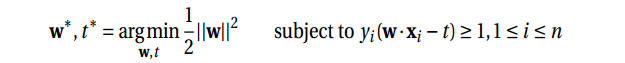
\includegraphics[width=.7\linewidth]{svm0.png}
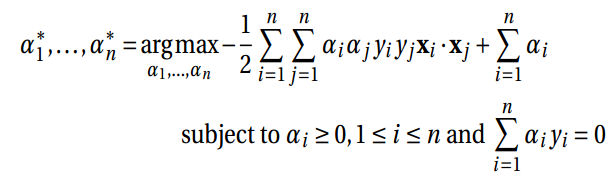
\includegraphics[width=.7\linewidth]{svm.png}\\
$w=\sum^n_{i=1}\alpha_iy_ix_i$
\\
\textbf{decision boundary} is defined only by the (typically few) support vectors from the training set - those that are nearest to the decision boundary (at the margin) Far examples  for which $\alpha_i = 0$ can be removed from the training set without affecting the learned decision boundary. And the weight vector w is merely a linear combination of the (typically few) support vectors. The threshold  can be found by solving m=1=wx-t for any support vector 
\\
\textbf{Soft Margin SVM} 
We introduce a slack variable  for each training example to account for margin errors. The \textbf{complexity parameter} C is a user-defined parameter that allows for a tradeoff between maximizing the margin (lower C) and minimizing the margin errors (higher C). Note that when C = 0, this gives no penalty to outliers -- which makes it equivalent to our basic linear classifier!  minimal-complexity (low C) soft margin classifier summarizes the classes by their class means in a way very similar to the basic linear classifier. In effect, these slack variables implement what was called \textbf{hinge loss}\\
 training examples divided into three cases:\\
$\alpha_i=0$ these are outside or on the margin, $C>\alpha_i>0$ these are the support vectors on the margin, $\alpha_i=C$ these are on or inside the margin.
\\
\textbf{Perceptron vs SVM} In the perceptron model, we iteratively learn the linear discriminant w, which is a linear combination of the misclassified input vectors. In SVM learning, we solve a constrained optimization problem. In both, the linear decision boundary is a linear combination of the training data points. In the perceptron, just the ones that get misclassified in the iterative training. In the SVM, just the (few) support vectors. Both have a dual form in which the dot product of training data points is part of the main computation. Perceptron and (basic) SVM learning only converge to a solution if the training data is linearly separable. If the data is not linearly separable, we can employ a soft margin SVM, where we introduce a slack variable. 
\subsection{non-linear \& probabilities}
We can adapt our linear methods to learn (some) nonlinear decision boundaries by transforming the data nonlinearly to a feature space in which is suited for linear classification. 
\\
\textbf{kernel trick} is a way of mapping features into another (often higher dimensional) space to make the data linearly separable, without having to compute the mapping explicitly. The dot product operation in a linear classifier x1x2 is replaced by a kernel function K(x1, x2) that computes the dot product of the values (x1, x2) in the new (linearly separable) space. \textbf{Assumption} achieving linear separation is worth the effort,  the dot product is the key computation. 
\\
\textbf{kernel svm} We can then replace the Gram matrix G with the kernel matrix
K, and use entries of K in the learning computation. After learning the $\alpha_i$  parameters, we can then classify a new instance x using $\sum^K_{i=1}\alpha_iy_iK(x,x_i)>t$ This sum is only over the support vectors, so it's an efficient computation
\\
\textbf{kernel functions} linear, polynomial $(x_1^Tx_2+c)^d$, Gaussian(RBF, $exp(-\|x_1-x_2\|^2/2\sigma^2)$, a measure of similarity between x1 and x2, scaled by $\sigma$, The larger $\sigma$ is, the more effect a distant point x will have)
\\
\textbf{choose a kernel function} \textbf{1.} Selecting a kernel function entails: \textbullet Choosing the function family (polynomial, RBF)\textbullet Determining the parameters of the function. \textbf{2. } using cross-validation, \textbf{applying machine learning to machine learning} \textbf{3. } Knowledge of the problem space can be helpful, Collected wisdom, In cases like this, try that kernel function. 
\textbf{probability}\\
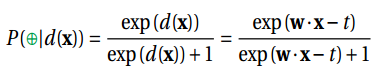
\includegraphics[width=.48\linewidth]{prob.png}
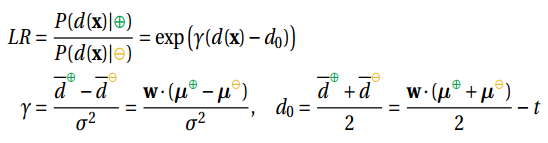
\includegraphics[width=.5\linewidth]{LR.png}
\end{document}
